\documentclass[a4paper,12pt,headsepline]{scrartcl}

%\part{title}
\usepackage[utf8]{inputenc}
\usepackage{graphicx}
\usepackage{caption,subcaption}
\usepackage[british]{babel}
\usepackage[T1]{fontenc}
\usepackage{geometry}
\usepackage{proof}
\geometry{left=3.5cm, right=2cm, top=2.5cm, bottom=2cm}
\usepackage{hyperref}
%\usepackage[hyphens,obeyspaces,spaces]{url}
\usepackage{fancybox}
\usepackage{amssymb,amsmath,amsthm}
\usepackage{gensymb}
\usepackage[linesnumbered,ruled,vlined,norelsize]{algorithm2e}
%\usepackage[bookmarksnumbered,pdftitle={\titleDocument},hyperfootnotes=false]{hyperref} 
\usepackage{color}
\usepackage{float}
\usepackage{enumerate}

%test
%\usepackage[backend=bibtex]{biblatex}
%\usepackage{filecontents}

%\addbibresource{ref.bib}

\restylefloat{figure}

% Makros
%\newenvironment{sketch}{\begin{proof}[Proof (Sketch)]}{\end{proof}}
%\newtheorem{theorem}{Theorem}
%\newtheorem{assumption}{Assumption}
%\newtheorem{lemma}{Lemma}
%\newtheorem{remark}{Remark}
%\newtheorem{definition}{Definition}
%\newtheorem{corollary}{Corollary}
\newcommand{\comment}[1]
{
  \begin{quotation}
    \textcolor{blue}{\underline{Edit:} #1}
  \end{quotation}
}
\newtheorem{aufgabe}{Aufgabe}
\newcommand{\Ex}[2]
{
	\setcounter{section}{#2}
	\section*{Übungsblatt #2 zu #1}
}
\newcommand{\TODO}[1]
{
  \begin{quotation}
    \textcolor{red}{\underline{TODO:} #1}
  \end{quotation}
}
% Zeichen 
\newcommand{\OO}{\ensuremath{\mathcal{O}}}
\newcommand{\ec}{\texttt{ec}}
\newcommand{\NP}{\call{NP}}
\newcommand{\call}[1]{\ensuremath{\mathcal{#1}}}

% neue Kopfzeilen mit fancypaket
\usepackage{fancyhdr} %Paket laden
\pagestyle{fancy} %eigener Seitenstil
\fancyhf{} %alle Kopf- und Fußzeilenfelder bereinigen
\fancyhead[L]{Benjamin \c Coban \\ Christoph Jabs}
\fancyhead[C]{Algorithmen und Komplexität \\ Blatt 1}
\fancyhead[R]{3526251 \\ 5567177}
\setlength{\headheight}{39pt}
\renewcommand{\headrulewidth}{0.4pt} %obere Trennlinie
%\fancyfoot[C]{\thepage} %Seitennummer
%\renewcommand{\footrulewidth}{0.4pt} %untere Trennlinie

\frenchspacing
\makeindex

% Pseudocode für Java
\usepackage{listings}
\lstset{numbers=left, numberstyle=\tiny, numbersep=5pt, keywordstyle=\color{black}\bfseries, stringstyle=\ttfamily,showstringspaces=false,basicstyle=\footnotesize,captionpos=b}
\lstset{language=java}

% Disable single lines at the start of a paragraph (Schusterjungen)
\clubpenalty = 10000
% Disable single lines at the end of a paragraph (Hurenkinder)
\widowpenalty = 10000
\displaywidowpenalty = 10000

\begin{document}

\begin{aufgabe}
\end{aufgabe}

\begin{enumerate}[a)]
	\item The runtime of the Algorithm 1 for the shortest path problem equals $\mathcal{O}(n\cdot m)$, where $n$ equals the number of vertices and $m$ equals the number of edges.
	\begin{proof}
		The initialization of the lengths runs in $\mathcal{O}(n)$. For the worst case scenario, for every length update a new shorter path will be revealed, until every vertex is finally evaluated ($\mathcal{O}(n)$). To find the newly revealed shortest path, it takes $\mathcal{O}(m)$ comparisons. Hence, the algorithm will run in $\mathcal{O}(n\cdot m)$ in the worst case and in $\mathcal{O}(\max\{n,m\})$ in best case.
	\end{proof}
	\item $A <_{\text{aymp}} B<_{\text{aymp}} E <_{\text{aymp}} C <_{\text{aymp}} D$
	\begin{proof}
		\begin{itemize}
			\item $A <_{\text{aymp}} B$
			\begin{align*}
				 2^{\sqrt{\log n}} = {2^{\log n}}^{\frac{1}{2}} = {2^{\frac{1}{2}}}^{\log n} = \sqrt{2}^{\log n}
			\end{align*}
			Also, the following holds. Let $f$ be a monotone increasing function and $c > 1$. Then:
			\begin{align*}
				\lim\limits_{\infty}\frac{c^f}{f} > 1
			\end{align*}
			\item $B <_{\text{aymp}} E$
			\begin{align*}
				2^{\sqrt{\log n}} < 2^{\sqrt{\log n \cdot \log n}} = n < 28n
			\end{align*}
			\item $E <_{\text{aymp}} C$
			\begin{align*}
				\log n^{\log n} = (2^{\log \log n})^{\log n}= n^{\log \log n}
			\end{align*}
			Therefore, every linear function out of $\mathcal{O}(n)$ will be outgrown by $C$.
			\item $C <_{\text{aymp}} D$
			\begin{align*}
				\mathcal{O}(2^{\log \log n}) \subset \mathcal{O}(2^n1)
			\end{align*}
		\end{itemize}
	\end{proof} 
\end{enumerate}
\newpage
\begin{aufgabe}
\end{aufgabe}

\begin{enumerate}
	\item 
	\item Consider the drawing of the following graph:
	\begin{figure}[H]
		\centering
		\begin{subfigure}{0.8\textwidth}
			\centering
			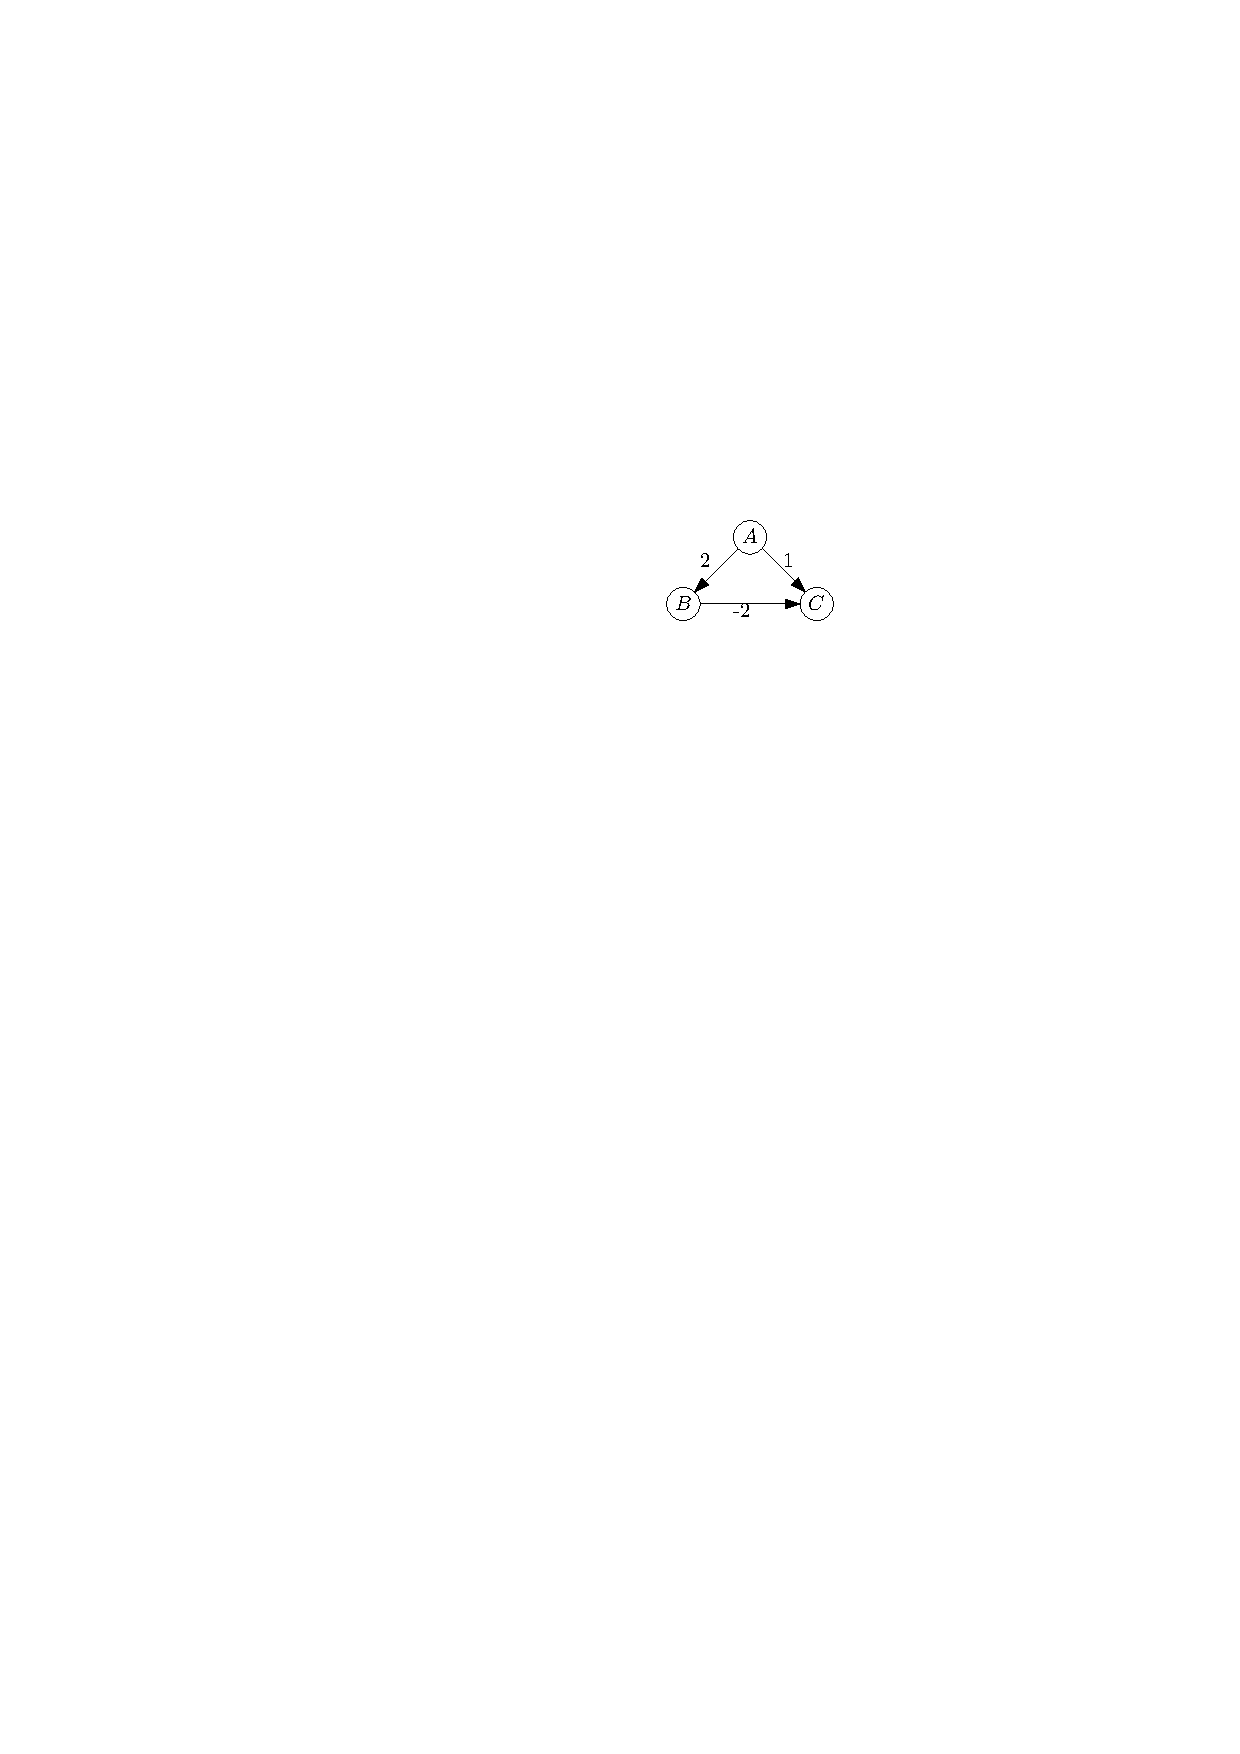
\includegraphics{22.pdf}
			\caption*{$\Gamma_G$}
		\end{subfigure}
	\end{figure}
	Here, the PQ will look as follows:
	\begin{quotation}
		\texttt{PQ = [(A,0),(C,$\infty$),(B,$\infty$)]}
	\end{quotation}
\texttt{Extract\_Min} returns and deletes \texttt{(A,0)}. Its neighbours will get updated to $PQ'$:
\begin{quotation}
	\texttt{PQ' = [(C,1),(B,2)]}
\end{quotation}
Next, $C$ will extracted since it is the minimum. But no edge from $C$ is left out of $PQ'$. The result will be:
\begin{align*}
	d[A] &= 0\\
	d[B] &= 2\\
	d[C] &= 1 \neq 0
\end{align*}
Therefore not the correct answer.
\end{enumerate}

\newpage
\begin{aufgabe}
\end{aufgabe}

\newpage
\begin{aufgabe}
\end{aufgabe}

\begin{enumerate}[a)]
	\item The height of a Fibonacci heap is in $\mathcal{O}(n)$ in the worst case.
	\begin{proof}
		Consider a chain of increasing elements $L$. Then, The first element can be interpreted as a root list with one element which has one child. This child has only one child and so on. Every element points to itself in a linked list. Therefore, $L$ can be interpreted as a valid Fibonacci Heap where the height is in $\mathcal{O}(|L|)$.
	\end{proof}
\end{enumerate}

\end{document}